\documentclass{article}
\usepackage[english]{babel}

\usepackage[letterpaper,top=1cm,bottom=2cm,left=3cm,right=3cm,marginparwidth=1.75cm]{geometry}
\usepackage{amsmath}
\usepackage{graphicx}
\usepackage[colorlinks=true, allcolors=blue]{hyperref}
\usepackage{newtxtext}
\usepackage{enumitem}
\usepackage{hyperref}
\usepackage{float}
\usepackage{wrapfig}
\usepackage{placeins}
\usepackage{caption}
\captionsetup[figure]{justification=centering}

\title {India's Essential Guide to Boycott China \\[1ex] \large Revision 1}
\author{Shaurya Bhardwaj}
\begin{document}

\maketitle

Despite the recent trends of ethical and sustainable practice the past two years have witnessed China's rapid occupation of the global export market by the allure of extraordinarily low prices. Rising political tensions have sparked international debates across various platforms raising questions about the ethical dilemmas of trade practices and the world's reliance on Chinese-manufactured goods. This scrutiny gave rise to the "Boycott China" movement. However, despite repeated efforts and rising trade tensions, India seems to be unable to break free of China's dependence.

\bigskip

Tensions first arose between British India and Qing dynasty of China over the Tibetan region.
The Sino-Indian War of 1962 erupted over territorial disputes along the Himalayan border. Chinese forces launched a surprise attack on Indian positions, leading to a brief and intense conflict. China emerged victorious, occupying strategic territories in Aksai Chin and Arunachal Pradesh. 
Since then border tensions with China rose leading to stand-off situations in 1967 and more recently in Doklam, 2017.

\bigskip

\section*{Understanding the dependence}

After the Galwan Valley incident [\hyperlink{link1}{1},\hyperlink{link2}{2}] on 15th June 2020, India banned 59 Chinese apps including the infamous TikTok. Shockingly, 2021 recorded a 50\% increase in Chinese imports to a value of over 92 billion USD. It seems like boycotting China had an opposite effect, as it was the highest growth recorded since 2007! 
\bigskip
\\
Fig.1 shows that from (2000-2010) China developed a strong hold on the Indian market, increasing by over 25 times in value in 10 years, from 1.6 billion in 2000 to 41 billion USD in 2010. Compare that to the growth in the last decade where the the imports were valued at 63 billion USD in 2020. Let’s look into the what caused this.

\begin{figure}[h]
    \centering
    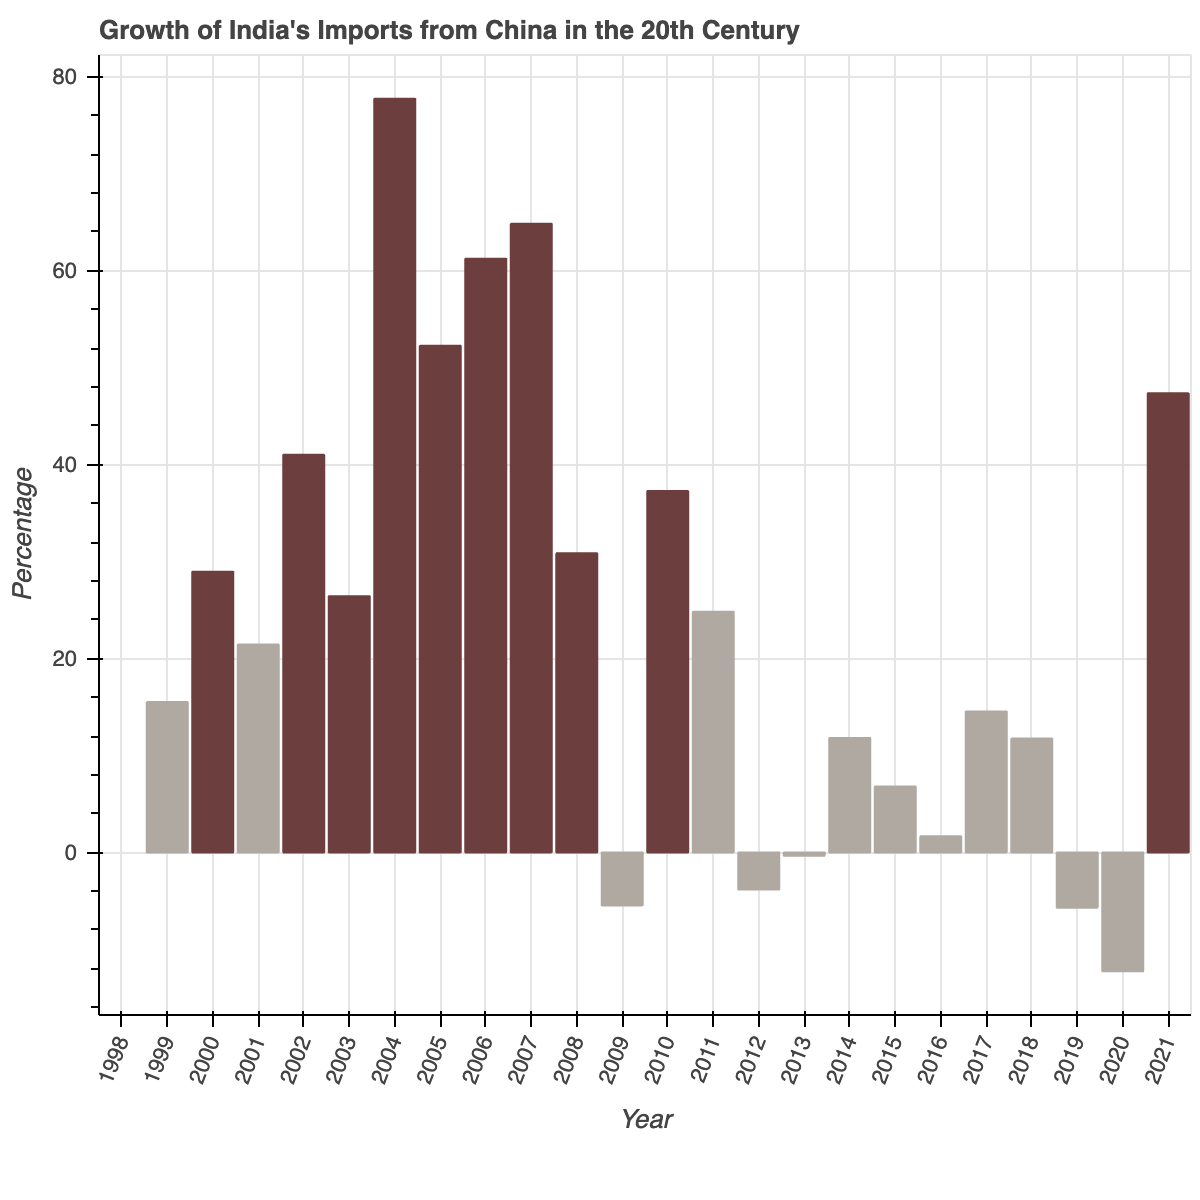
\includegraphics[width=0.48\textwidth]{ind_chn_imports.png} % Replace "example-image" with the filename of your image
    \captionsetup{skip=0pt,font=small} % Adjust the skip as needed
    \caption{Percentage growth of Chinese imports 1998-2021. In the years 1998-2010 (excluding The Great Recession of 2009 ) China developed a strong hold in the Indian market recording increasing growth in export rates yearly. In 2010-2020 growth was slower and irregular and but in 2021, growth spiked to ~50\%}
\end{figure}

\newpage
    \begin{table}[htbp]
        \centering
        \caption{Comparison of timelines of Indian and Chinese policies on Globalisation and Infrastructure policies}
        \begin{tabular}{|p{3cm}|p{6cm}|p{6cm}|}
            \hline
            \textbf{} & \textbf{China} & \textbf{India} \\
            \hline
            Globalisation &
            \begin{itemize}[nosep , left=0pt , topsep=0pt]
                \item In late 1970’s Den Xiaoping setup Special Economic Zones (SEZ’s) opening up to Foreign Investment.
                \item Gradual reduction of trade barriers. As part of its accession to the WTO in 2001, tariff reductions in sectors such as agriculture, manufacturing, and services.
            \end{itemize}
            &
            \begin{itemize}[left=0pt , topsep=0pt]
                \item In 1991, India faced an Economic Crisis and the New Economic Policy was introduced under PM Narsimha Rao and Finance Minister Manmohan Singh.It promoted Industrial growth and integrated India to the global economy.
            \end{itemize} \\
            \hline
            Infrastructure &
            \begin{itemize}[nosep , left=0pt , topsep=0pt]
                \item From 1978-1990, the Four Modernizations policy focused on developing 4 key sectors including agriculture, industry, defence, science and technology.
                \item In 2013 Belt and Roads Initiative to develop transport facilities for efficient supply chains.
            \end{itemize} &
            \begin{itemize}[nosep , left=0pt , topsep=0pt]
                \item In 1998, the National Highway Development Programme was launched without significant industrial development.
                \item In 2005, Jawaharlal Nehru National Urban Development program was launched
                \item 2014 - Make in India - promoting Manufacturing in India
                \item In 2017 the National Infrastructure Pipeline aimed at investing in the critical Infrastructure projects

            \end{itemize}  \\
            % Add more rows as needed
            \hline
        \end{tabular}
    \end{table}
\paragraph{}
Poorly timed ineffective policies majorly contributed to the doomed decade of growing dependence. In China, setup of SEZ’s started in the late 1970’s almost 10 years before India but trade barriers were only gradually reduced 20 years later in the 2000’s after substantial infrastructural development.
On the other hand, India's disordered and unregulated measures to fix the economic crisis, caused unsupervised removal of trade barriers exposing the unprepared Indian markets to direct competition from advanced Chinese counterparts. An accessible cheap market made the situation unfavourable for any further industry development in India. 
Bureaucracy also played a role in making these infrastructural projects less effective and disjoint with each other. The co-dependence between liberalisation of trade and infrastructural reforms weighed on each other causing India to rely on an external source, rather than itself.


\section*{What all are we importing?}

\begin{figure}[htp]
    \centering
    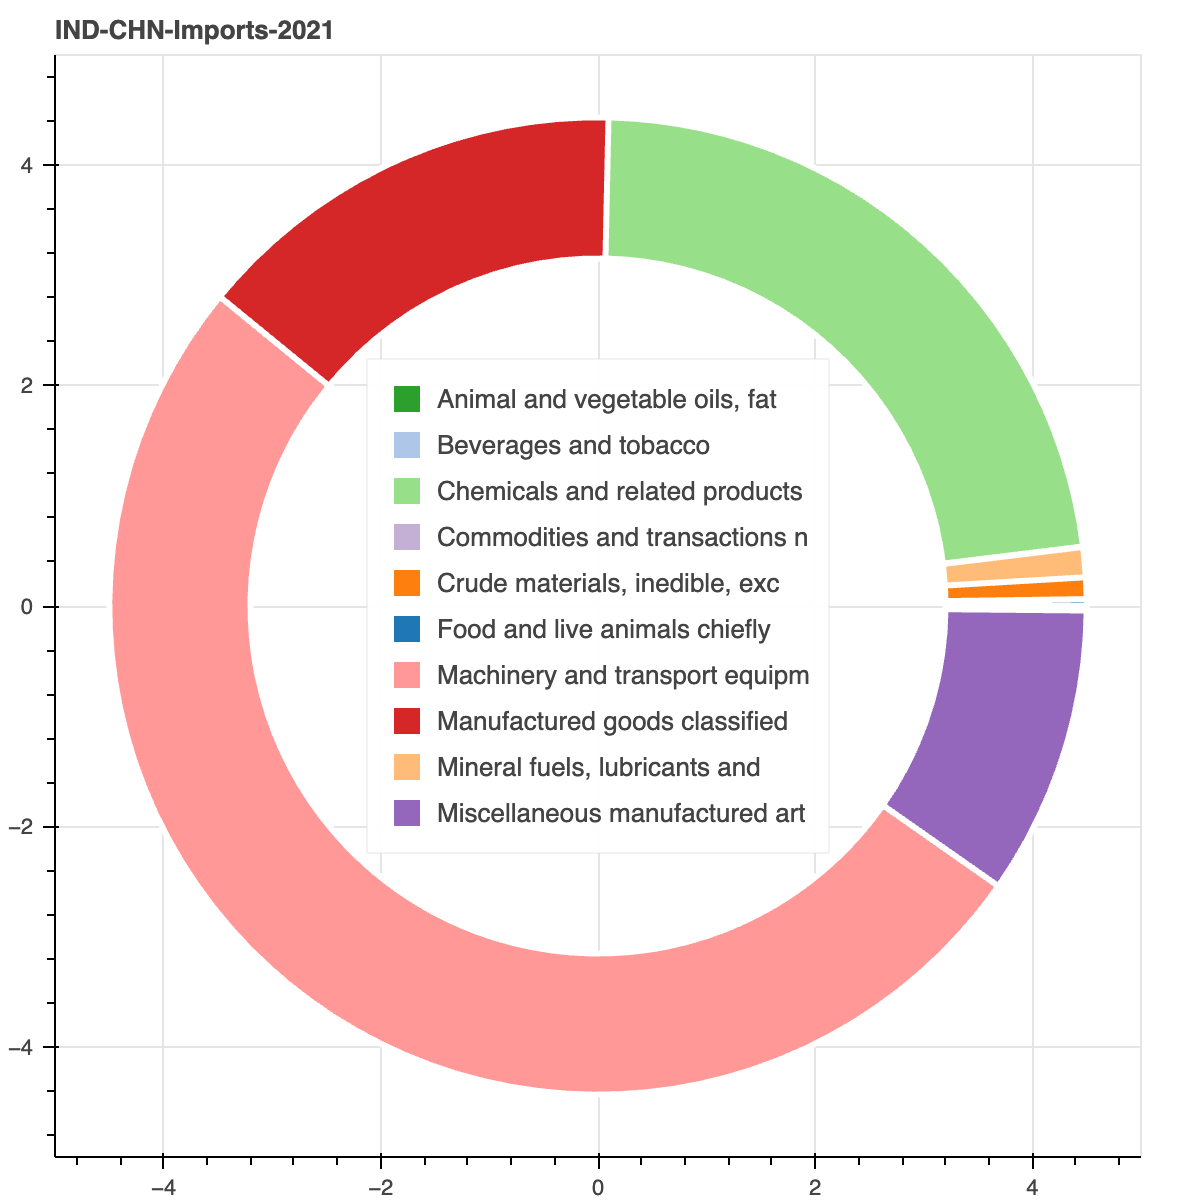
\includegraphics[width=0.48\textwidth]{ind_chn_imports_2021.png} % Replace "example-image" with the filename of your image
    \captionsetup{skip=0pt,font=small} % Adjust the skip as needed
    \caption{Breakdown of India's 92.8 billion USD Chinese Imports into 10 key SITC subgroups. Major imports include Electronic Machinery(50\%), Miscellaneous Manufactures(25\%) and Chemicals(23\%)}
\end{figure}


Of the total value of 93 billion USD Chinese imports into India, about 50\% was invested in Machines and Transport equipment, which through the last 2 decades, has remained fairly constant in proportion.
Fig.3 shows the composition of the ~47 billion USD imports in machinery in 2021, where Electrical Machinery and apparatus account for 32\% including diodes, transistors and other semiconductor-based products which is the top import, while Telecommunication devices and Office Machines and general industrial machinery account for 50\% of remaining total.

Manufactured articles comprise another quarter, and about 23\% are Chemical imports. Several articles[\hyperlink{link3}{3},\hyperlink{link4}{4}] talk about the dependence of India’s pharmaceutical exports on Chinese manufactured Active Pharmaceutical Ingredients (or API's).  
India supplied 2.65\% of the total 834 billion USD value of Medicinal and pharmaceutical exports in the world (~22 billion USD) while it imported only 2.14 billion USD from China(fig.4). 

\begin{figure}[htp]
\centering
\begin{minipage}{.5\textwidth}
  \centering
  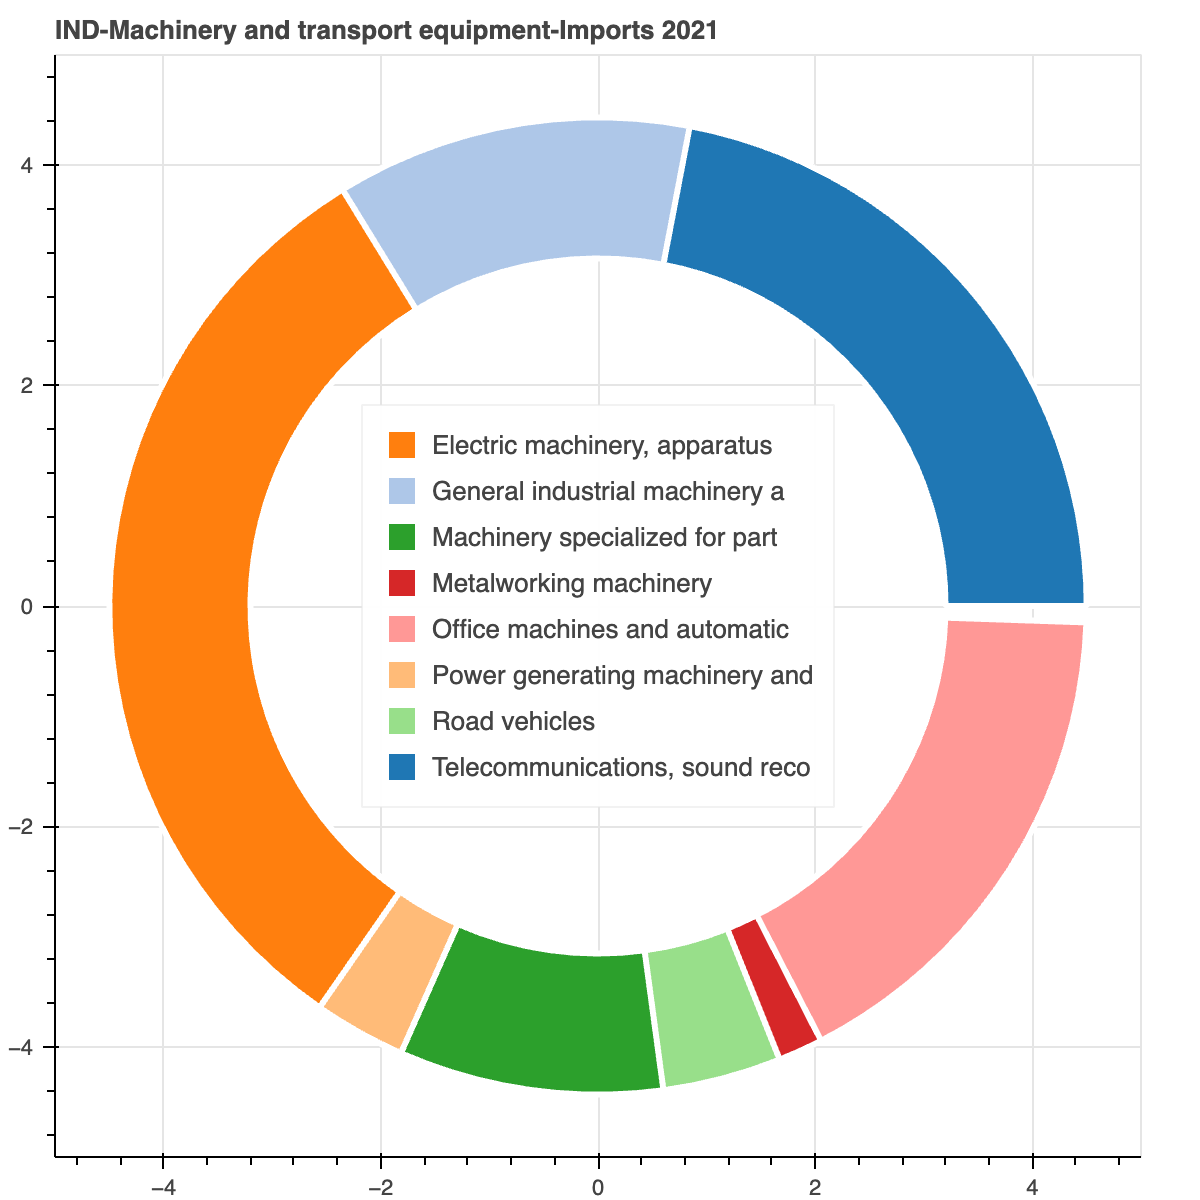
\includegraphics[width=.7\linewidth]{ind_chn_imports_machines.png}
  \captionsetup{skip=0pt,font=small} % Adjust the skip as needed
    \caption{Breakdown of India's 47 billion USD imports of Chinese Machinery and Transport equipment in 2021. Major imports include Semiconductor Devices(32\%), Telecommunications equipment(22\%) and Office Machinery(17\%)}
  \label{fig:test1}
\end{minipage}%
\begin{minipage}{.5\textwidth}
  \centering
  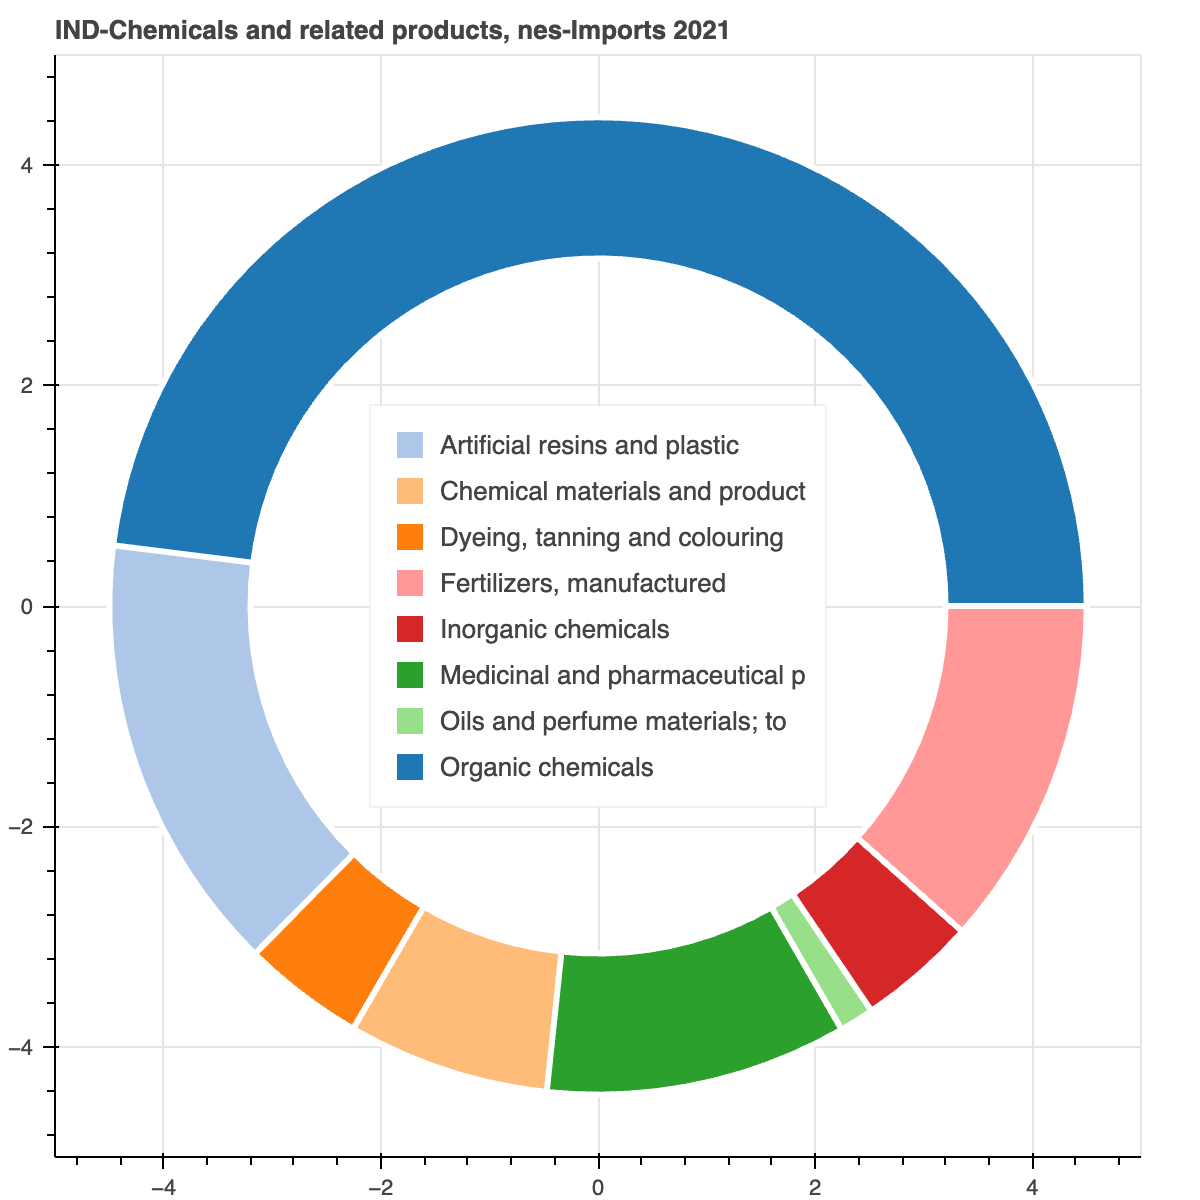
\includegraphics[width=.7\linewidth]{ind_chn_imports_chemicals.png}
  \captionsetup{skip=0pt,font=small} % Adjust the skip as needed
    \caption{Breakdown of India's 21 billion USD imports of Chinese Chemicals in 2021. Major imports include Organic Chemicals(48\%), Artificial resins and Plastic(14.7\%) and Fertilizers(11.6\%)}
  \label{fig:test2}
\end{minipage}
\end{figure}


\section*{Why this is concerning?}
    \begin{itemize}[nosep , left=0pt , topsep=0pt]
        \item It is a cause of macroeconomic instability
            \paragraph{}
            These stark features highlight India’s one-sided import dependence on China which has created a mammoth trade imbalance between the two countries, contributing to a growing current account deficit (CAD). Despite China’s growing trade surplus, articles talk about how this surplus is a result of structural imbalances in China’s economy and not real economic prosperity [\hyperlink{link5}{5},\hyperlink{link6}{6}]. This causes a sluggish increase in imports, making it a losing game for India. The IMF prescribes reforms to reduce trade imbalances which China has continually ignored and unlike any other exporters(Fig.5).[\hyperlink{link7}{7}]
            Indian export industries that rely on Chinese raw products bear risk the of supply chain disruptions, especially during geopolitical challenges. 
            \begin{figure}[h]
                \centering
                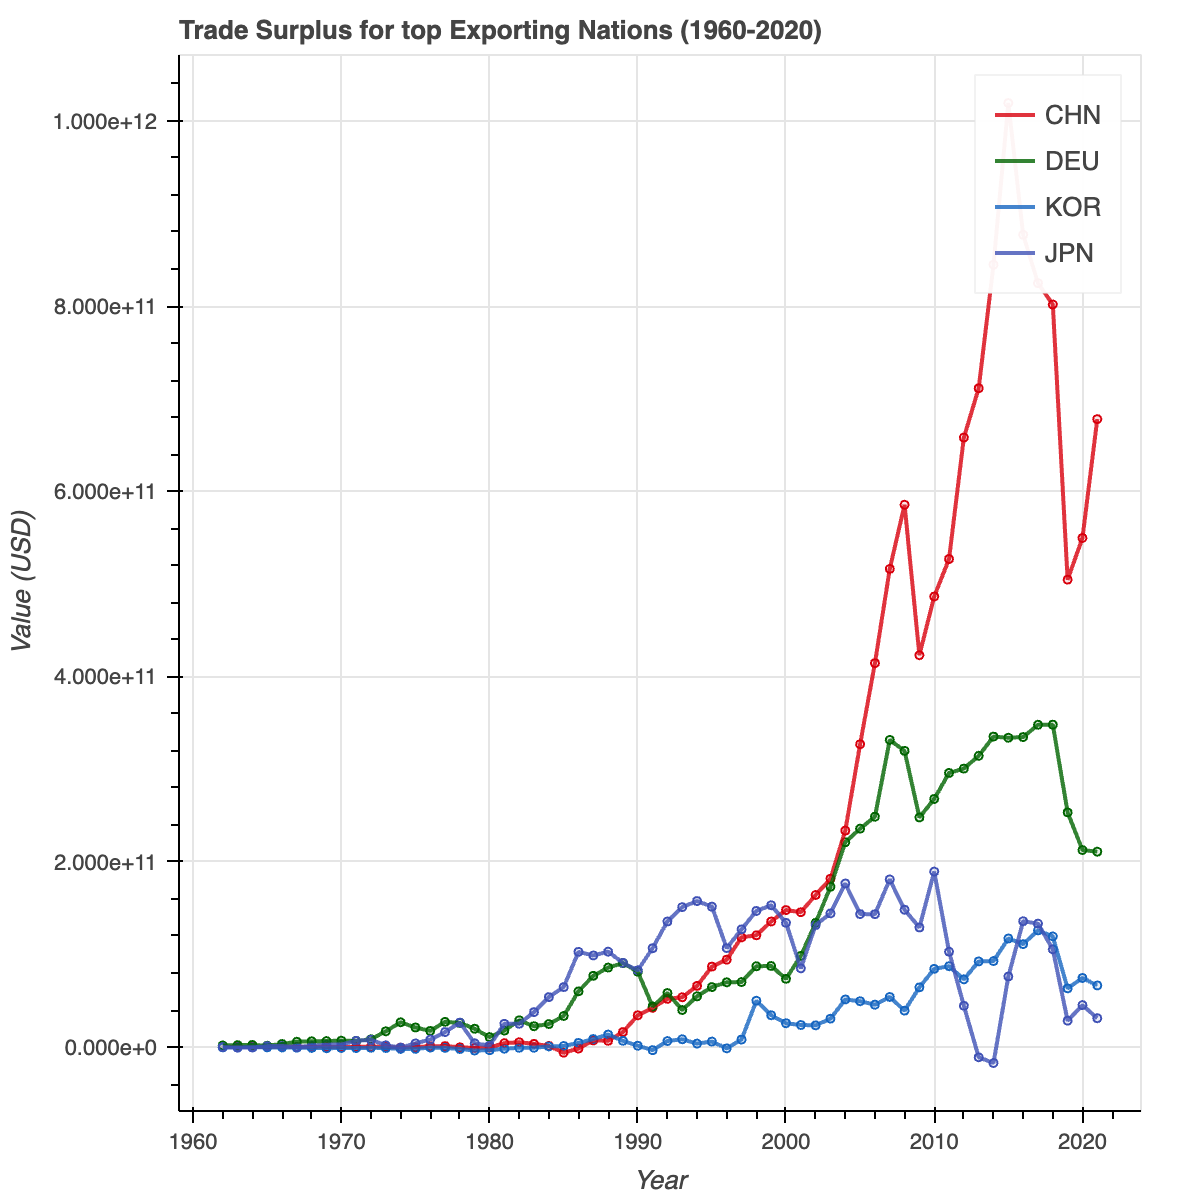
\includegraphics[width=0.4\textwidth]{trade_surplus_graph.png} % Replace "example-image" with the filename of your image
                  \captionsetup{skip=0pt,font=small} % Adjust the skip as needed
                    \caption{Trade Surpluses of major exporters China, Germany, Japan and South Korea) over time. China's skyrocketing trade surplus despite IMF's(International Monetary Fund) guidelines disrupts global macroeconomic stability.}
                \label{fig:example}
            \end{figure}
\bigskip            
        \item It inhibits the development of the Indian industry
            \paragraph{}
            Indeed, India could not resist the appeal of low Chinese prices achieved through efficient systems, industrial development and an undervalued Chinese currency.
            This has resulted in the Indian manufacturing industry’s inability to invest in itself creating a vicious cycle of dependency is established from which the Indian domestic market is being unable to escape.
            This is especially problematic in the context of the India-China relationship, as trade with an aggressor [\hyperlink{link1}{1},\hyperlink{link2}{2}] and political threat is akin to financially funding your own attacks, providing indirect permission for future behaviour and molding an increasingly weak position on the international stage. 
\bigskip
        \item It is a blackbox which provides us cheap products and strong viruses at the cost of human rights
            \paragraph{}
            Further, check out this page [\hyperlink{link8}{8}] with a list of Chinese goods along with the type of exploitation method used for manufacture. A quick search pops up countless articles about the labour abuse practices in China. A paper titled “Negative consequences of using exports to earn foreign exchange”explains the environmental degradation, widening of development gaps and loss of real wealth that is concealed by the magnitude of economic growth.[\hyperlink{link9}{9}]
            China is also the only major economy to have recorded a positive GDP growth in 2020(Fig.6). Which further proves Covid-19 being a Chinese bioweapon[\hyperlink{link10}{10},\hyperlink{link11}{11}]. Its true that we can’t say for sure what is going on behind the curtains and that is why such a dependancy is even more problematic.
            The low prices are not only a result of economic development also underhand financial manipulations and forced illegal labour.

            \begin{figure}[h]
                \centering
                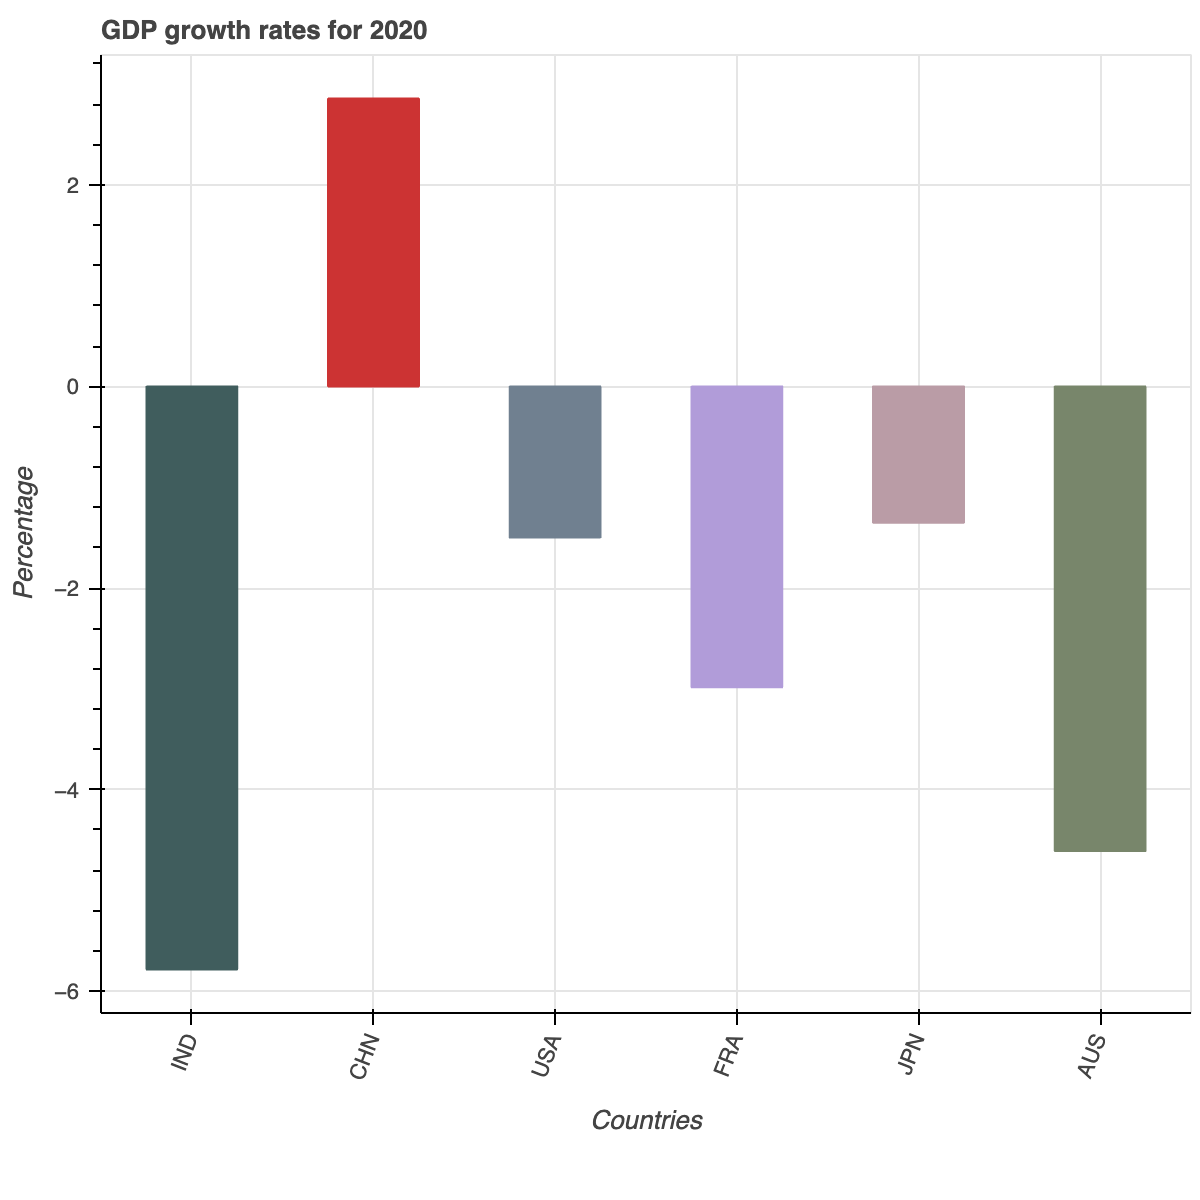
\includegraphics[width=0.5\textwidth]{2020_gdp_growth_rates.png} % Replace "example-image" with the filename of your image
                \captionsetup{skip=0pt,font=small} % Adjust the skip as needed
                    \caption{COVID-19 caused negative GDP's for all major economies except one. I will leave it for you to guess who the lucky one was}
                \label{fig:example}
            \end{figure}

            
    \end{itemize} 
\section*{What can we do now?}
The harsh reality is that the solving it is not easy because of the prices of Chinese products. A majority buyers of Chinese products are the middle class or businesses where costs need to be cut while maintaining quality. However, there are ways to decrease and gradually remove the dependence.
\bigskip
\begin{itemize}[nosep , left=0pt , topsep=0pt]
        \item Moving to alternate markets 
            \paragraph{}
            Short term solutions encourage businesses and startups to turn to other growing markets in the world. First we must address upcoming markets in the Electrical Machinery sector. 
            For example, Taiwan is the second largest exporter of semiconductor products. Vietnam controls ~11\% of world exports of telecommunication products with growing companies like the Viettel Group. China has a strong hold on the market for office machinery with companies like HP, Canon and Epson and controls ~44\% of the world exports for which Taiwanese companies like Acer prove to be a strategic option.
            Considering the proximity and share of Electronics exports supplied by Taiwan, it has proven to be a key upcoming market for India to invest in. Stronger trade alliances should be formed to facilitate shifting to Taiwanese products easily.
\bigskip
        \item Investment in industry development
            \paragraph{}
            In the end there are no shortcuts. We need to do it the hard way by investing in our industries, developing them to global standards in terms of prices and quality. 
            Schemes like “Make in India” and “National Infrastructure Pipeline” need to be effectively implemented. 
            Forms of trade barriers and tax reforms need to be made to regulate the prices and flow of Chinese imports. Provision of tax incentives and government aid to set up native and foreign industries in India.
\bigskip
        \item Investment in our services exports
            \paragraph{}
            The 1980’s were characterised by the rise of the services sector of India which currently accounts for 40\% of Indias total exports and 4\% of Global services trade. 1990’s trade reforms paved the way for India’s service sector to expand exponentially.
            \\
            \begin{figure}[htp]
            \centering
            \begin{minipage}{.5\textwidth}
              \centering
              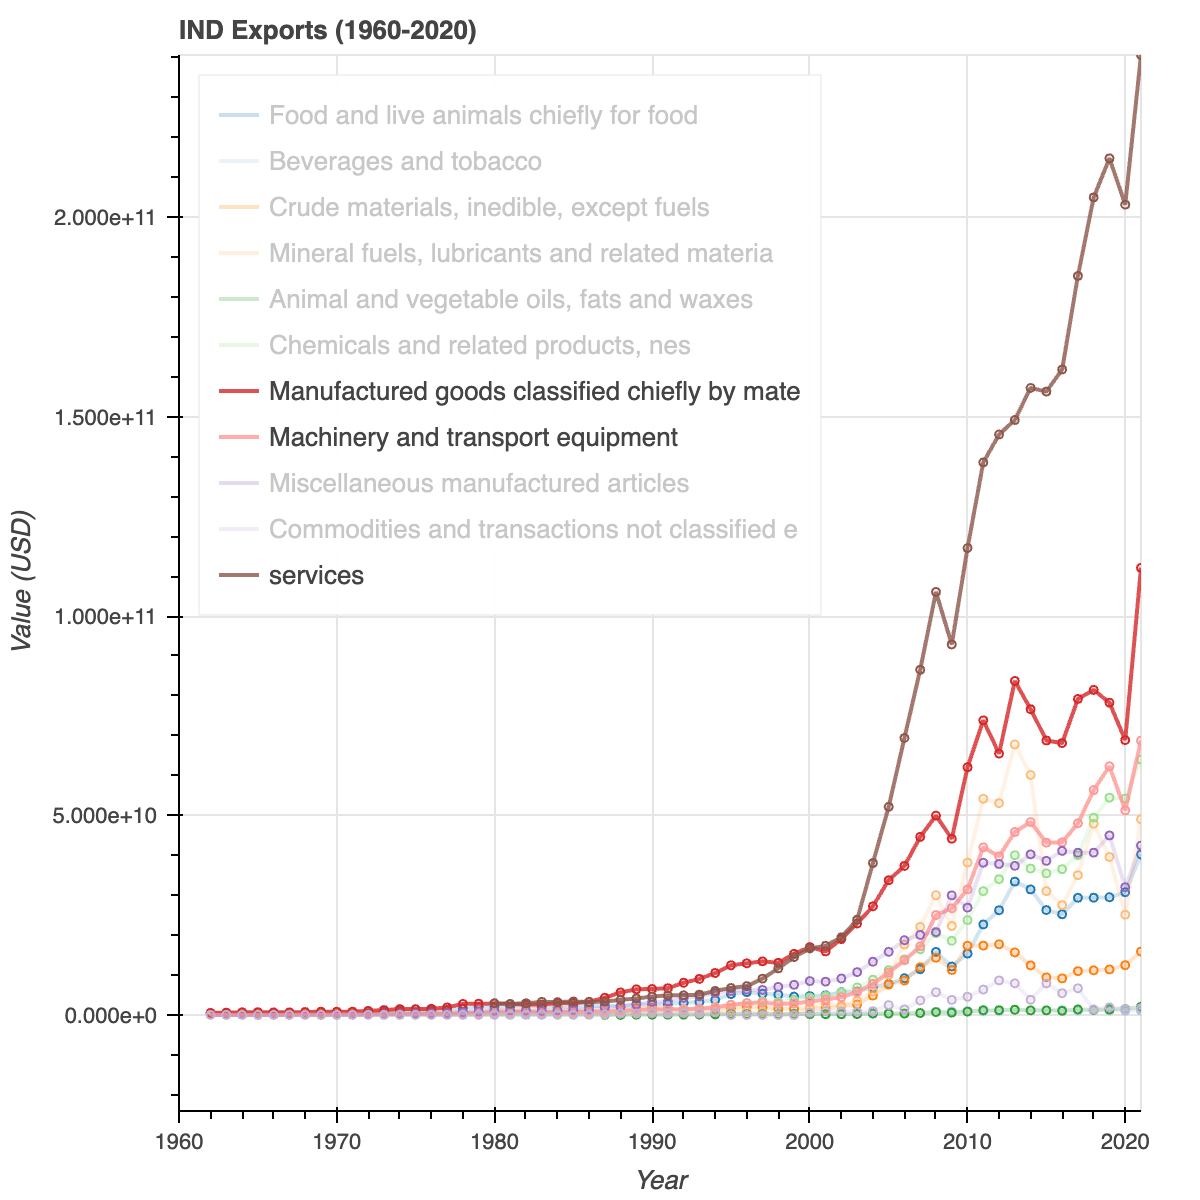
\includegraphics[width=.9\linewidth]{ind_exports_1960_2020.png}
              \captionsetup{skip=0pt,font=small} % Adjust the skip as needed
                \caption{Indian sector wise exports 1962-2021
                \\The services sector emerged in 1980 and quickly rose to become a high value trade for India. In 20th century the growth has left all merchandise trade way behind and this calls for further investment to harness India's advantages in this sector.}
              \label{fig:test1}
            \end{minipage}%
            \begin{minipage}{.5\textwidth}
              \centering
              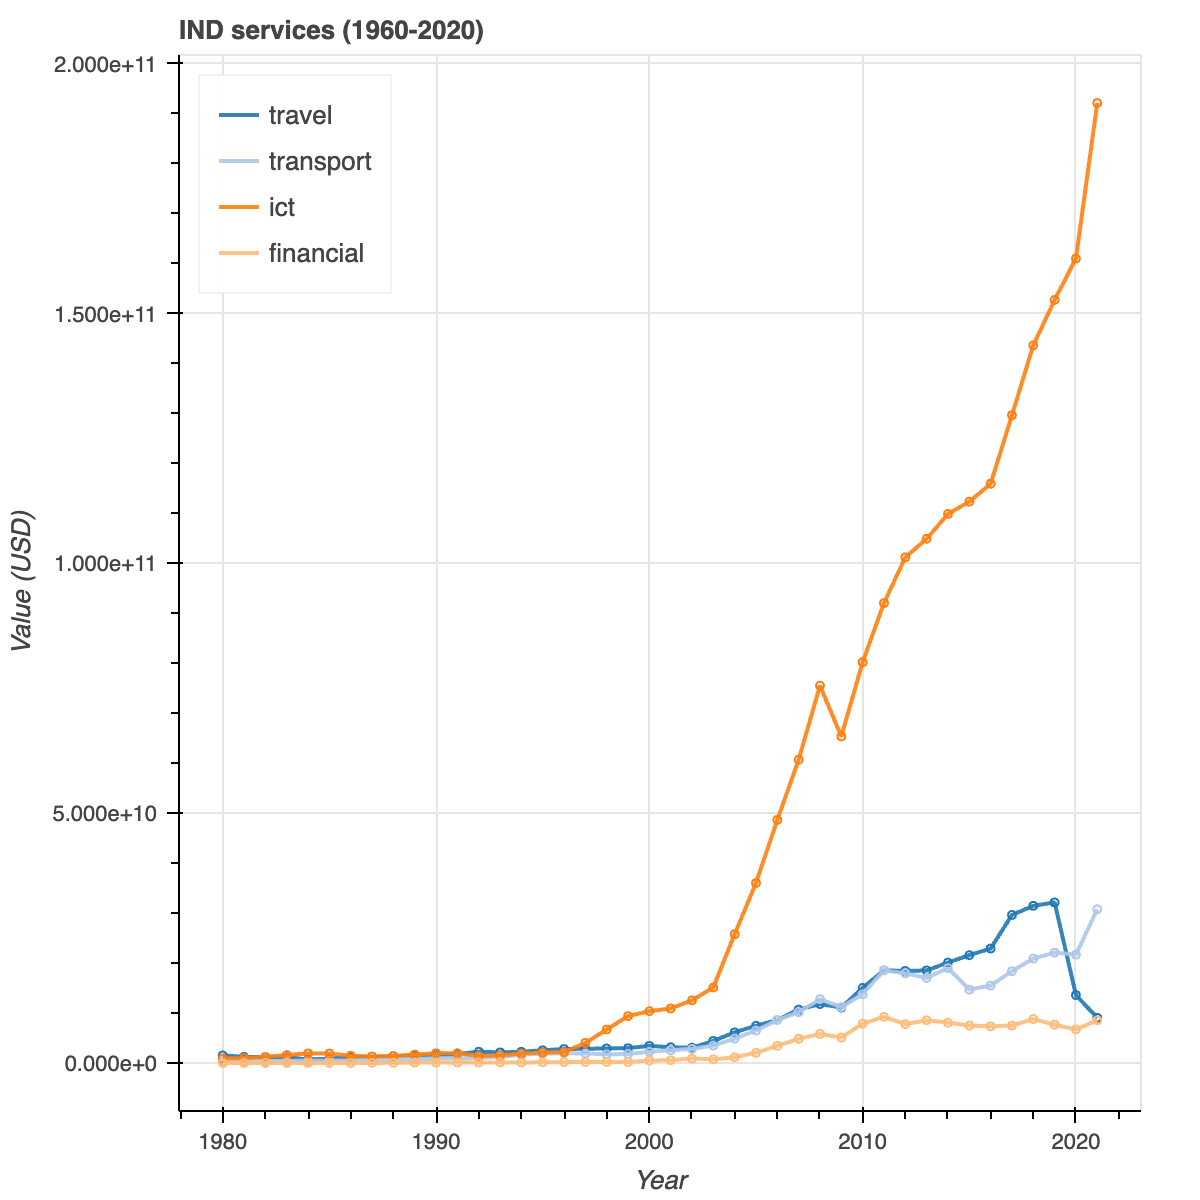
\includegraphics[width=.9\linewidth]{ind_services_1960_2020.png}
              \captionsetup{skip=0pt,font=small} % Adjust the skip as needed
                \caption{Indian Exports in the services sector 1980-2021
                \\Investing Information and Communications Technology services are the way forward for India, as they have driven surpluses and contributed to growth unlike any other trades.}
              \label{fig:test2}
            \end{minipage}
            \end{figure}
            \\
            Amongst the different subsections Information and communications technology services have grown the most. Services export provide a high and consistent trade surplus to India. This is particularly beneficial for improving the value of the Indian Currency as well as generating revenue. Thus, instead of only trying to solve the issue directly, a further promotion of services export to utilise India’s large population in favour of development will contribute to reduced dependencies.

    \end{itemize} 

\section*{Conclusion}
Hence, India's trade relationship with China is marked by a deep-seated dependency, tainted by a history of political tensions and a recent push for the "Boycott China" movement. Despite efforts to diversify and strengthen domestic production, India's continuous and significant reliance on Chinese imports, highlights a pressing challenge. Overcoming this issue calls for a multi-faceted strategy, including exploring new trade partnerships, investing in domestic industries and leveraging India's ICT services sector, to reduce dependency and promote economic self-reliance amidst ongoing geopolitical challenges.

\newpage

\section*{References}
\hypertarget{link1}{[1] \href{https://www.bbc.com/news/world-asia-india-53076781}{https://www.bbc.com/news/world-asia-india-53076781}}
\\
\hypertarget{link2}{[2] \href{https://www.ndtv.com/india-news/china-has-intruded-423-metres-into-indian-territory-in-the-galwan-valley-2253916}{https://www.ndtv.com/india-news/china-has-intruded-423-metres-into-indian-territory-in-the-galwan-valley-2253916}}
\\
\hypertarget{link3}{[3] \href{https://www.cnbc.com/2022/05/27/india-needs-to-fill-china-gaps-to-become-the-pharmacy-of-the-world.html}{https://www.cnbc.com/2022/05/27/india-needs-to-fill-china-gaps-to-become-the-pharmacy-of-the-world.html}}
\\
\hypertarget{link4}{[4] \href{https://www.financialexpress.com/business/sme-msme-eodb-despite-being-worlds-pharmacy-why-indian-pharma-is-dependent-on-china-for-bulk-drugs-2386143/}{https://www.financialexpress.com/business/sme-msme-eodb-despite-being-worlds-pharmacy-why-indian-pharma-is-dependent-on-china-for-bulk-drugs-2386143/}}
\\
\hypertarget{link5}{[5] \href{https://carnegieendowment.org/chinafinancialmarkets/88098}{https://carnegieendowment.org/chinafinancialmarkets/88098}}
\\
\hypertarget{link6}{[6] \href{https://cepr.org/voxeu/columns/real-causes-chinas-trade-surplus}{https://cepr.org/voxeu/columns/real-causes-chinas-trade-surplus}}
\\
\hypertarget{link7}{[7] \href{https://www.imf.org/en/Blogs/Articles/2017/07/28/global-imbalances-avoiding-a-tragedy-of-the-commons}{https://www.imf.org/en/Blogs/Articles/2017/07/28/global-imbalances-avoiding-a-tragedy-of-the-commons}}
\\
\hypertarget{link8}{[8] \href{https://www.dol.gov/agencies/ilab/reports/child-labor/list-of-goods-print?items_per_page=10&combine=china}{https://www.dol.gov/agencies/ilab/reports/child-labor/}}
\\
\hypertarget{link9}{[9] \href{https://www.sciencedirect.com/science/article/pii/S2590051X23000382}{https://www.sciencedirect.com/science/article/pii/S2590051X23000382}}
\\
\hypertarget{link10}{[10] \href{https://economictimes.indiatimes.com/news/international/world-news/covid-19-was-created-as-a-bioweapon-by-china-wuhan-researcher/articleshow/101346204.cms?}{https://economictimes.indiatimes.com/news/international/world-news/covid-19-was-created-as-a-bioweapon-by-china-wuhan-researcher/articleshow/101346204.cms?}}
\\
\hypertarget{link11}{[11] \href{https://www.bbc.com/news/world-asia-china-57268111}{https://www.bbc.com/news/world-asia-china-57268111}}
\\
\hypertarget{link12}{[12] \href{https://carnegieendowment.org/2010/10/30/is-world-too-dependent-on-chinese-economy-pub-41850}{https://carnegieendowment.org/2010/10/30/is-world-too-dependent-on-chinese-economy-pub-41850}}
\\
\hypertarget{link13}{[13] \href{https://economictimes.indiatimes.com/news/economy/policy/government-working-on-steps-to-cut-import-dependence-on-china-boost-manufacturing-sources/articleshow/76449657.cms?from=mdr}{https://economictimes.indiatimes.com/news/economy/policy/government-working-on-steps-to-cut-import-dependence-on-china-boost-manufacturing-sources/articleshow/76449657.cms?from=mdr}}
\\
\hypertarget{link14}{[14] \href{https://www.bloomberg.com/news/articles/2023-02-14/china-s-economic-bonanza-from-record-trade-surplus-is-fading}{https://www.bloomberg.com/news/articles/2023-02-14/china-s-economic-bonanza-from-record-trade-surplus-is-fading}}
\\
\hypertarget{link15}{[15] \href{https://economy-finance.ec.europa.eu/economic-and-fiscal-governance/macroeconomic-imbalance-procedure_en}{ https://economy-finance.ec.europa.eu/economic-and-fiscal-governance/macroeconomic-imbalance-procedure}}
\\
\hypertarget{link16}{[16] \href{ https://www.livemint.com/economy/trade-deficit-with-china-widens-despite-move-to-cut-dependency-11658252467641.html}{ https://www.livemint.com/economy/trade-deficit-with-china-widens-despite-move-to-cut-dependency-11658252467641.html}}
\\
\hypertarget{link17}{[17] \href{ https://www.aei.org/op-eds/were-too-dependent-on-china-for-too-many-critical-goods-especially-medicine/}{ https://www.aei.org/op-eds/were-too-dependent-on-china-for-too-many-critical-goods-especially-medicine/}}
\\


\end{document}
